\begin{figure*}[!t]
    \centering
    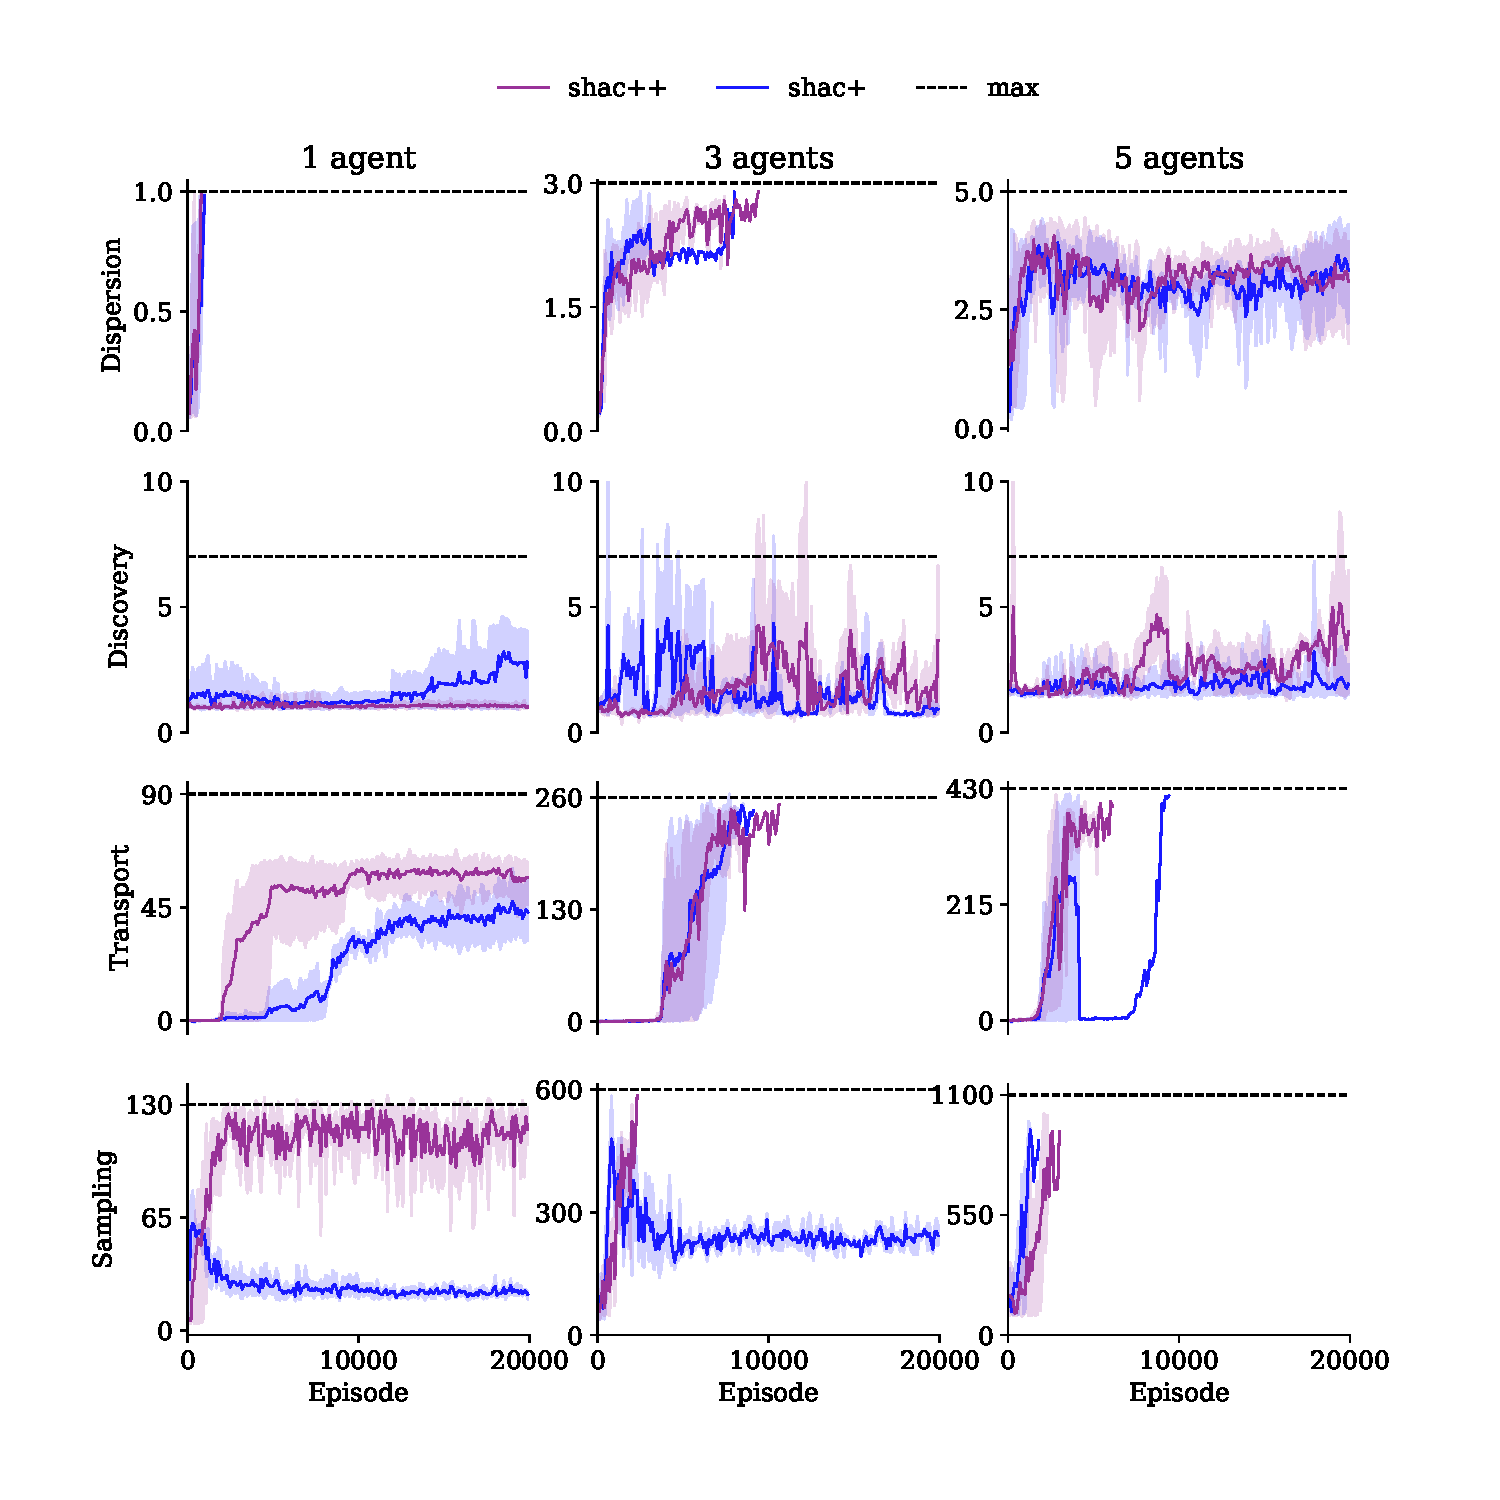
\includegraphics[width=\textwidth]{figs/ablation-transformer.pdf}
    \caption{Comparison between \fname{} with and without transition network, labelled \fnamer{}, for increasing number of agents for Dispersion, Transport, Discovery, and Sampling scenarios.}
    \label{fig:ablation}
\end{figure*}




\section{Ablation Study}\label{sect:ablation}
While we mainly focus on replacing both the reward and transition function with neural networks, we also investigate the effect of replacing only the latter. 

In fact, the transition function is the most complex component to replace as it requires modeling with precision the observations obtained from the environment after a number of $H$ actions from each agent. Avoiding the need of such network lightens the algorithm but it reintroduce the need for a differentiable environment.

Fig.~\ref{fig:ablation} summarizes the results. Most notably, using the true transition function does not appear to provide any significant advantage in terms of reward achieved. In fact, in some cases, we report better results for \fname{}, namely in Fig.~\ref{fig:transport-ablation-1-mlp}. 
